\documentclass[11pt]{article}
\usepackage[T1]{fontenc}
\usepackage[utf8]{inputenc}
\usepackage{lmodern,microtype}
\usepackage[margin=1in]{geometry}
\usepackage{amsmath,amssymb,mathtools,bm,amsthm}
\usepackage{graphicx,booktabs,tabularx,array}
\usepackage{xcolor,enumitem,caption,float}
\usepackage[section]{placeins}
\usepackage{tikz}
\usetikzlibrary{arrows.meta,positioning,calc}
\usepackage[numbers,sort&compress]{natbib}
\usepackage{xurl}
\usepackage{hyperref}
\usepackage[nameinlink,noabbrev]{cleveref}

\hypersetup{
  colorlinks=true,
  linkcolor=blue!45!black,
  citecolor=green!35!black,
  urlcolor=blue!55!black,
  pdftitle={Exact Low-Dimensional Quantum Hodology}
}
\captionsetup{font=small,labelfont=bf}
\setlist{leftmargin=1.6em}
\setlength{\emergencystretch}{2em}
\allowdisplaybreaks
\graphicspath{{results/}{results/figures/}{results/qutrit-phase/}}

\newtheorem{theorem}{Theorem}[section]
\newtheorem{proposition}[theorem]{Proposition}
\newtheorem{lemma}[theorem]{Lemma}
\newtheorem{corollary}[theorem]{Corollary}
\theoremstyle{definition}
\newtheorem{definition}[theorem]{Definition}
\newtheorem{example}[theorem]{Example}
\theoremstyle{remark}
\newtheorem{remark}[theorem]{Remark}

\newcommand{\C}{\mathbb C}
\newcommand{\R}{\mathbb R}
\newcommand{\Z}{\mathbb Z}
\newcommand{\E}{\mathbb E}
\newcommand{\Prob}{\mathbb P}
\newcommand{\Tr}{\operatorname{Tr}}
\newcommand{\rank}{\operatorname{rank}}
\newcommand{\diag}{\operatorname{diag}}
\newcommand{\ket}[1]{\lvert #1\rangle}
\newcommand{\bra}[1]{\langle #1\rvert}
\newcommand{\braket}[2]{\langle #1\mid #2\rangle}
\newcommand{\proj}[1]{\lvert #1\rangle\!\langle #1\rvert}
\newcommand{\Dens}{\mathcal D}
\newcommand{\cE}{\mathcal E}
\newcommand{\one}{\mathbf 1}
\newcommand{\doi}[1]{\href{https://doi.org/#1}{doi:#1}}

\title{\textbf{Exact Low-Dimensional Quantum Hodology}\\
\large From Qubit Action Histories to a Two-Dimensional Qutrit Phase Chart}
\author{RL Experiments Project\\
\small A pedagogical companion to the exact-construction notebooks}
\date{August 2026}

\begin{document}
\maketitle

\begin{abstract}
Can nine spatial goals be realized by a qubit or qutrit, even though neither
system has nine mutually orthogonal states? The answer is yes, but the meaning
of realization matters. Hilbert-space dimension bounds perfect one-shot
discrimination; it does not bound the number of distinct quantum states,
controlled histories, or goals. This chapter develops that distinction from
first principles and gives three exactly soluble models.

First, four nonorthogonal qubit states form a projective Pauli orbit whose
optimal control cost is exactly the Euclidean metric of one square cell.
Second, two rationally independent qubit phase rotations give a faithful
action of $\Z^2$; nine nonorthogonal orbit goals have the exact open
$3\times3$ Manhattan word metric, and unit-cost retry instruments give exact
Euclidean distance in expectation. This construction is algebraically exact
but physically fragile because the orbit is dense on a one-dimensional Bloch
circle. Third, a qutrit supplies two independent relative phases. Carefully
chosen commuting generators have Fubini--Study covariance
$\frac{3}{16}I_2$; an order-11 orbit contains 121 separated states, and nine
of them form an exact rank-two Euclidean control-cost chart.

Along the way we prove the one-shot orthogonality obstruction, finite-automaton
universality, the Bellman criterion for exact hitting costs, Schoenberg's
Euclidean-distance criterion, and a general projective-orbit retry theorem.
Numerical experiments validate every closed-form result and expose the
recognition, tolerance, topology, and memory-provenance limitations. The
result is both an introduction to the mathematics and a precise foundation
for asking when hodological distance can become ordinary physical space.
\end{abstract}

\noindent\textbf{Keywords:} quantum instruments; reinforcement learning;
stochastic shortest path; goal geometry; hodological space; Euclidean distance
matrix; qubit; qutrit; Fubini--Study metric

\tableofcontents
\newpage

\section{The question, stated carefully}
\label{sec:motivation}

The guiding idea is operational. For an agent, a goal that can be achieved by
a short and reliable sequence of interventions is near; a goal that requires
many uncertain interventions is far. The resulting space of goal-directed
difficulty is a \emph{hodological space}. It need not initially resemble
physical space. It may be directed, asymmetric, high-dimensional, or partly
stored in the agent's memory.

The project asks whether a special regime can occur in which:
\begin{enumerate}
  \item many place-like goals share a common control repertoire;
  \item optimal all-pairs difficulty behaves like distance;
  \item the distance matrix embeds in two or three Euclidean dimensions;
  \item action sequences become trajectories through recovered coordinates;
  \item the geometry is carried by the controlled physical process rather than
  merely written into a classical goal counter.
\end{enumerate}



Earlier constructions used nine orthogonal basis states of a
nine-dimensional Hilbert space as nine places. Such a model makes
localization simple, but it raises a natural challenge: is dimension nine
essential, or can a qubit or qutrit support the same goal geometry using
nonorthogonal states and richer sequence goals?

There are two superficially contradictory facts:
\begin{itemize}
  \item A $d$-dimensional Hilbert space contains continuously many pure states.
  A qubit is not limited to two possible states.
  \item No more than $d$ nonzero states can be identified perfectly by one
  common, error-free, one-shot measurement.
\end{itemize}

The entire subject lies in understanding which fact is relevant to a
particular meaning of place. This document separates several meanings, proves
exact possibility and impossibility results, and then uses simulation to audit
the gap between algebraic exactness and operational robustness.

\subsection{A map of the argument}

\Cref{sec:quantum} reviews quantum states, instruments, and measurement
backaction. \Cref{sec:states} separates physical, predictive, and
goal-progress state. \Cref{sec:control} introduces stochastic-shortest-path
control and \cref{sec:distance} gives the exact Euclidean embedding test.
\Cref{sec:obstructions} proves what low Hilbert dimension does and does not
forbid. \Cref{sec:retry} then converts group metrics into exactly soluble
quantum control problems.

The constructions follow in increasing strength. The qubit Pauli square in
\cref{sec:pauli} is the minimal nondegenerate cell. The irrational-phase
qubit in \cref{sec:irrational} scales to the requested $3\times3$ patch but is
fragile. The qutrit phase model in \cref{sec:qutrit} supplies a genuine
two-dimensional state manifold and a finite separated orbit.
\Cref{sec:experiments} presents the numerical checks, while
\cref{sec:conditions} organizes the emerging necessary-and-sufficient
conditions.

\section{Quantum preliminaries}
\label{sec:quantum}

\subsection{States and pure-state rays}

A finite quantum system is described externally by a Hilbert space
$\mathcal H\simeq\C^d$. A density operator is a positive semidefinite,
unit-trace matrix
\begin{equation}
  \rho\succeq0,\qquad \Tr\rho=1.
  \label{eq:density}
\end{equation}
Pure states have rank one and may be written
$\rho=\proj{\psi}$ with $\braket{\psi}{\psi}=1$. Multiplication of
$\ket{\psi}$ by a global phase does not change $\rho$:
\begin{equation}
  \proj{e^{i\gamma}\psi}=\proj{\psi}.
\end{equation}
The physical pure state is therefore a \emph{ray}, not a particular vector.
This is why projective rather than ordinary unitary representations naturally
appear below.

The real affine dimension of the density-operator space is $d^2-1$. A qubit
has a three-dimensional Bloch ball of states,
\begin{equation}
  \rho=\frac12(I+\bm r\cdot\bm\sigma),\qquad \|\bm r\|_2\le1,
  \label{eq:bloch}
\end{equation}
and pure states lie on its two-dimensional boundary sphere. Thus
Hilbert-space dimension is not a count of possible states.

\subsection{POVMs and quantum instruments}

A measurement outcome is represented by a positive operator-valued measure
(POVM) $\{E_o\}$:
\begin{equation}
  E_o\succeq0,\qquad \sum_oE_o=I,\qquad
  \Prob(o\mid\rho)=\Tr(E_o\rho).
  \label{eq:povm}
\end{equation}
A POVM specifies probabilities but not the post-measurement state. An
\emph{instrument} specifies both. For action $a$ and reported outcome $o$,
\begin{equation}
  \cE_o^a(\rho)=\sum_kK^a_{o,k}\rho K^{a\dagger}_{o,k},
  \qquad
  \sum_{o,k}K^{a\dagger}_{o,k}K^a_{o,k}=I.
  \label{eq:instrument}
\end{equation}
The outcome probability and conditional update are
\begin{equation}
  p(o\mid\rho,a)=\Tr\cE_o^a(\rho),\qquad
  \rho'=\frac{\cE_o^a(\rho)}{p(o\mid\rho,a)}.
  \label{eq:instrument-update}
\end{equation}
The completeness relation is the first check for every Kraus construction in
this chapter \cite{kraus1983,nielsen2010}.

A unitary action is a one-outcome instrument with $K=U$ and
$U^\dagger U=I$. A random-unitary retry instrument has two outcomes,
\begin{equation}
  K_{\rm s}=\sqrt p\,U,\qquad
  K_{\rm f}=\sqrt{1-p}\,I.
  \label{eq:basic-retry}
\end{equation}
It is valid because the Kraus Gram sum is $pI+(1-p)I=I$. Its special
importance is operational: success applies $U$, failure leaves the conditional
state unchanged, and the agent observes which occurred.

\subsection{Physical distance is not control distance}

For later interpretation, distinguish fidelity, trace distance, and
Fubini--Study distance:
\begin{align}
 F(\rho,\sigma)
 &=\left(\Tr\sqrt{\sqrt\rho\,\sigma\sqrt\rho}\right)^2,
 \label{eq:fidelity}\\
 D_{\rm tr}(\rho,\sigma)
 &=\frac12\|\rho-\sigma\|_1,
 \label{eq:trace-distance}\\
 d_{\rm FS}(\psi,\phi)
 &=\arccos|\braket{\psi}{\phi}|.
 \label{eq:fs-distance}
\end{align}
For pure states,
$F=|\braket{\psi}{\phi}|^2$ and
$D_{\rm tr}=\sqrt{1-F}$. These quantify physical overlap or statistical
distinguishability. They need not agree with \emph{control cost}. A central
lesson below is that four physical states can form a regular tetrahedron under
state overlap while forming a square under optimal action cost
\cite{holevo2011,bengtsson2017}.

\section{Three state spaces and where geometry can hide}
\label{sec:states}

\subsection{Physical, predictive, and goal-progress state}

The physical state is the density operator $\rho_t\in\Dens(\mathcal H)$.
The agent in an operational reinforcement-learning problem need not be given
$\rho_t$; it may be a hidden state used only by the simulator.

The agent observes a history
\begin{equation}
  h_t=(a_0,o_0,\ldots,a_{t-1},o_{t-1}).
  \label{eq:history}
\end{equation}
Two histories are predictively equivalent when no future controlled
experiment can distinguish them:
\begin{equation}
 h\sim_{\rm pred}h'
 \Longleftrightarrow
 p(\bm o\mid h,\bm a)=p(\bm o\mid h',\bm a)
 \quad\text{for every future }(\bm a,\bm o).
 \label{eq:predictive-equivalence}
\end{equation}
An equivalence class is an operational causal or predictive state. In a known
Markovian quantum model, the posterior density operator is sufficient, but a
learner may instead compress history into a recurrent representation.

A sequence goal is a language over action--outcome symbols. A regular
language is recognized by a deterministic finite automaton (DFA),
\begin{equation}
  q_{t+1}=\delta(q_t,a_t,o_t),\qquad q_t\in Q,
  \label{eq:dfa}
\end{equation}
with accepting set $F_g\subseteq Q$. The Markov state of the
goal-conditioned problem is the product
\begin{equation}
  (\rho_t,q_t)\in\Dens(\mathcal H)\times Q.
  \label{eq:product-state}
\end{equation}
The automaton size $|Q|$ is not bounded by $d$. A recurrent network can store
similar progress continuously, but changing the representation does not remove
the information requirement.

\begin{remark}[The provenance question]
When an experiment displays a two-dimensional embedding, ask what would remain
if the quantum instrument were replaced by an identity channel while the goal
automaton were left intact. Geometry that survives unchanged is geometry of
external task memory, not evidence that the quantum process carries space.
\end{remark}

\section{Hodological cost as stochastic shortest path}
\label{sec:control}

\subsection{From goal pursuit to expected cost}

Let $S$ be a finite operational state set. At state $i$, action $a$ costs
$c(i,a)>0$ and produces state $j$ with probability $P_a(i,j)$. For goal
$g$, define the first hitting time
\begin{equation}
  \tau_g=\inf\{t\ge0:S_t=g\}
\end{equation}
and the policy cost
\begin{equation}
  D^\pi(i,g)=
  \E_\pi\left[
    \sum_{t=0}^{\tau_g-1}c(S_t,A_t)
    \,\middle|\,S_0=i
  \right].
  \label{eq:policy-cost}
\end{equation}
The hodological distance candidate is
\begin{equation}
  D(i,g)=\inf_\pi D^\pi(i,g).
  \label{eq:optimal-cost}
\end{equation}
This turns easy and hard into expected intervention units. It also makes
clear that distance is a property of states, actions, costs, outcomes, and
goal semantics together.

\subsection{Deriving the Bellman equation}

Suppose $i\ne g$ and the first selected action is $a$. The agent immediately
pays $c(i,a)$, reaches $j$ with probability $P_a(i,j)$, and then faces the
same optimization problem. Conditioning on that first transition gives
\begin{equation}
  Q_g(i,a)=c(i,a)+\sum_jP_a(i,j)D(j,g).
  \label{eq:action-cost}
\end{equation}
Choosing the least expensive first action yields
\begin{align}
  D(g,g)&=0,\label{eq:bellman-goal}\\
  D(i,g)&=\min_a\left[
    c(i,a)+\sum_jP_a(i,j)D(j,g)
  \right],\qquad i\ne g.
  \label{eq:bellman}
\end{align}
For a proper stochastic-shortest-path problem, each goal is reached almost
surely under at least one policy and improper policies have infinite or
inferior cost. Under these conditions the optimal column $D(\cdot,g)$ is the
minimal nonnegative solution of \cref{eq:bellman}
\cite{bellman1957,puterman1994,bertsekas1991}.

\begin{proposition}[Bellman realizability]
\label{prop:bellman}
A proposed finite hitting-cost matrix is dynamically realizable by a specified
proper control problem if and only if each goal column satisfies
\cref{eq:bellman-goal,eq:bellman} and a minimizing proper policy exists.
\end{proposition}

\begin{proof}
Necessity follows by conditioning an optimal policy on its first action.
For sufficiency, select a minimizing action in each nonterminal state.
Repeated substitution expresses the proposed value as expected accumulated
cost plus expected residual value. Properness makes the residual vanish at
the hitting time, so the selected policy attains the proposed value. Every
alternative first action has value no smaller by the Bellman inequality, and
induction extends this to every policy.
\end{proof}

\subsection{Why hitting cost need not be a distance}

In a general controlled process, $D(i,j)$ can differ from $D(j,i)$.
Information gathering can be source dependent; irreversible actions can make
one direction cheaper; risk penalties can violate additivity. Ordinary metric
geometry requires
\begin{equation}
\begin{split}
 D(i,j)&=D(j,i),\qquad D(i,i)=0,\\
 D(i,j)&>0\quad(i\ne j),\\
 D(i,k)&\le D(i,j)+D(j,k).
\end{split}
\label{eq:metric-axioms}
\end{equation}
Failure of these conditions is not necessarily an error. It says that the
appropriate geometry is directed, information-augmented, or nonmetric.

\section{When is a finite cost matrix exactly Euclidean?}
\label{sec:distance}

\subsection{The double-centering construction}

Suppose $D=[D_{ij}]$ is a symmetric $N\times N$ distance matrix. If unknown
coordinates $x_i\in\R^k$ exist, then
\begin{equation}
 D_{ij}^2=\|x_i\|^2+\|x_j\|^2-2x_i^\top x_j.
 \label{eq:squared-distance}
\end{equation}
Translation does not affect distances, so assume $\sum_i x_i=0$. Define
\begin{equation}
 J=I-\frac1N\one\one^\top.
 \label{eq:centering}
\end{equation}
Multiplying the squared-distance matrix on both sides by $J$ removes the two
norm terms in \cref{eq:squared-distance}, leaving
\begin{equation}
  B=-\frac12J(D\circ D)J.
  \label{eq:schoenberg-gram}
\end{equation}

\begin{theorem}[Schoenberg's finite Euclidean criterion]
\label{thm:schoenberg}
A symmetric hollow matrix $D$ is the distance matrix of points in
$\R^k$ if and only if
\begin{equation}
  B\succeq0,\qquad \rank B\le k,
  \label{eq:schoenberg}
\end{equation}
where $B$ is given by \cref{eq:schoenberg-gram}
\cite{schoenberg1935,gower1966}.
\end{theorem}

\begin{proof}
If coordinates exist, the derivation above gives $B=XX^\top$, which is
positive semidefinite and has rank at most $k$. Conversely, if
$B=V\Lambda V^\top$ has nonnegative eigenvalues and rank $r\le k$, set
$X=V_r\Lambda_r^{1/2}$. Then $B=XX^\top$. Reversing
\cref{eq:squared-distance} recovers the original distances, so the rows of
$X$ are the required coordinates.
\end{proof}

\subsection{Classical multidimensional scaling}

The constructive half of the theorem is classical multidimensional scaling
(MDS). Positive eigenvalues of $B$ give coordinates. Negative eigenvalues
signal that the proposed distances are not exactly Euclidean. More than $k$
positive eigenvalues means exact embedding needs more than $k$ dimensions.

For approximate data, normalized raw stress is
\begin{equation}
 \operatorname{stress}(X)=
 \sqrt{
 \frac{\sum_{i<j}(\|x_i-x_j\|-D_{ij})^2}
      {\sum_{i<j}D_{ij}^2}
 }.
 \label{eq:stress}
\end{equation}
Low stress is useful evidence; zero stress together with
\cref{eq:schoenberg} is an exact certificate.

\begin{corollary}[Finite exact classification]
\label{cor:classification}
For a specified finite operational control problem, exact Euclidean
hodological geometry in $\R^k$ is equivalent to:
\begin{enumerate}
  \item proper Bellman realizability;
  \item symmetry and the metric axioms; and
  \item a positive-semidefinite Schoenberg Gram matrix of rank at most $k$.
\end{enumerate}
\end{corollary}

This classifies the cost matrix. It does not prove that actions are local,
that the agent can localize itself, or that the geometry survives noise.

\section{What low dimension forbids---and what it does not}
\label{sec:obstructions}

\subsection{Finite-automaton universality}

\begin{proposition}[Automaton universality]
\label{prop:automaton}
Let $G=(V,E)$ be any finite directed graph with positive edge costs. If goal
recognition may use an unrestricted finite automaton, a physical Hilbert space
of dimension $d=1$ can realize the shortest-path hodological geometry of
$G$ exactly.
\end{proposition}

\begin{proof}
Create one automaton state $q_v$ per vertex. For each edge $e=(v,w)$ provide
an action $a_e$ that changes $q_v$ to $q_w$ when legal and assign it the edge
cost. Let every physical action be the one-dimensional identity channel with
one deterministic outcome. Goal $g_w$ accepts at $q_w$. The Bellman equation
of the controller is exactly the shortest-path recursion on $G$, while the
physical system does nothing.
\end{proof}

Unit action cost does not rescue the claim. An integer-cost edge can be
replaced by a chain of auxiliary automaton states, and rational costs can be
implemented by retry processes. Therefore a plotted goal grid is not by itself
evidence of a physical spatial structure.

\subsection{Perfect one-shot recognition}

\begin{proposition}[Orthogonality obstruction]
\label{prop:orthogonality}
Suppose states $\rho_1,\ldots,\rho_N$ must be identified without error by one
common POVM $\{E_i\}_{i=1}^N$:
\begin{equation}
  \Tr(E_i\rho_j)=\delta_{ij}.
  \label{eq:perfect-discrimination}
\end{equation}
Their supports are mutually orthogonal. Consequently $N\le d$.
\end{proposition}

\begin{proof}
For $i\ne j$, positivity and $\Tr(E_i\rho_j)=0$ imply that $E_i$ vanishes on
the support of $\rho_j$. Meanwhile,
$\Tr(E_j\rho_j)=1$ and $0\preceq E_j\preceq I$ imply that $E_j$ acts as the
identity there. The support of $\rho_j$ is thus contained in the unit
eigenspace of $E_j$ and in the kernel of every $E_i$ with $i\ne j$. Distinct
supports are orthogonal, and their dimensions sum to at most $d$.
\end{proof}

For pure states the proof is especially transparent:
$E_i\ket{\psi_i}=\ket{\psi_i}$ and
$E_i\ket{\psi_j}=0$ imply
\begin{equation}
 \braket{\psi_j}{\psi_i}
 =\bra{\psi_j}E_i\ket{\psi_i}=0.
\end{equation}
An adaptive finite measurement tree acting on one copy is still one POVM when
all branches are collected, so adaptivity does not evade the bound. Repeated
fresh preparations or persistent history change the premise.

\subsection{Reversibility, commuting directions, and boundaries}

A channel with a completely positive trace-preserving inverse on the whole
matrix algebra is unitary. Exact reversible memoryless translations must
therefore be unitary channels. A maximal connected commuting subgroup of
projective qubit unitaries has one phase direction. A qutrit has two independent
relative phases, so $d=3$ is minimal for a smooth two-dimensional commuting
phase manifold of the kind built in \cref{sec:qutrit}.

This does \emph{not} imply that a qubit cannot encode $\Z^2$. A countable
faithful subgroup can be dense in its phase circle; that exceptional
construction is \cref{sec:irrational}. It is algebraically two-coordinate but
not a robust two-dimensional manifold.

A reversible action on a finite set is a permutation, so repeated homogeneous
translation produces cycles rather than an open boundary. An exact finite open
grid must break boundary homogeneity, use irreversible boundary actions, store
boundary position elsewhere, or appear as a patch of a larger periodic or
continuous space. The qutrit construction uses the last option.

\subsection{Why local lattice actions do not give exact Euclidean cost}

Four unit-cost axial moves yield Manhattan distance. Adding unit-cost
diagonals yields Chebyshev distance. Pricing a unit diagonal at $\sqrt2$
gives the octile metric, which is exact at offsets $(1,0)$ and $(1,1)$ but not
at $(2,1)$:
\begin{equation}
  1+\sqrt2\ne\sqrt5.
\end{equation}
An exact finite Euclidean all-pairs metric therefore needs a sufficiently rich
action repertoire, a continuous control limit with a Riemannian action cost,
or a different definition of difficulty.

\section{The projective-orbit retry theorem}
\label{sec:retry}

The next theorem is the common engine behind the exact Euclidean examples.

\begin{theorem}[Projective-orbit retry construction]
\label{thm:retry}
Let $G$ be a finite or countable group with a left-invariant metric $d_G$,
rescaled so that
$\min_{h\ne e}d_G(e,h)=1$. Suppose $G$ has a projective unitary
representation $U:G\to PU(d)$ and a fiducial density operator $\rho_0$ with
distinct orbit labels:
\begin{equation}
 U_g\rho_0U_g^\dagger=U_h\rho_0U_h^\dagger
 \quad\Longrightarrow\quad g=h.
 \label{eq:distinct-orbit}
\end{equation}
For each $h\ne e$, define
\begin{equation}
 K_{\rm s}^{(h)}=\sqrt{p_h}\,U_h,\qquad
 K_{\rm f}^{(h)}=\sqrt{1-p_h}\,I,\qquad
 p_h=\frac1{d_G(e,h)}.
 \label{eq:retry-instrument}
\end{equation}
If goal $g$ means that the accumulated successful group product equals $g$,
then the optimal expected number of unit-cost interventions from $x$ to $g$
is exactly
\begin{equation}
  D(x,g)=d_G(x,g).
  \label{eq:retry-result}
\end{equation}
\end{theorem}

\begin{proof}
The instrument is valid because
\begin{equation}
 K_{\rm s}^{(h)\dagger}K_{\rm s}^{(h)}
 +K_{\rm f}^{(h)\dagger}K_{\rm f}^{(h)}
 =p_hI+(1-p_h)I=I.
\end{equation}
Failure leaves the group coordinate at $x$; success changes it to $hx$.
Retry the direct displacement $h=gx^{-1}$. The number of attempts is geometric
with mean
\begin{equation}
 \E T_h=\frac1{p_h}=d_G(e,h)=d_G(x,g),
\end{equation}
so optimal cost is no larger than the metric distance.

For the lower bound define $V(x)=d_G(x,g)$. The one-step Bellman expression
for any $h$ is
\begin{equation}
 1+(1-p_h)V(x)+p_hV(hx).
\end{equation}
The triangle inequality and left invariance imply
\begin{equation}
 V(x)-V(hx)\le d_G(x,hx)=d_G(e,h)=\frac1{p_h}.
\end{equation}
Rearranging shows that the Bellman expression is at least $V(x)$. No action,
adaptive policy, or mixture can do better, while direct retry attains $V$.
\end{proof}

\begin{remark}[What the theorem does and does not explain]
The theorem proves exact optimality, but it places the desired metric in the
success probabilities. It is an analytic benchmark, not yet a derivation of
the Euclidean norm from simpler physics. The deeper inverse-design question is
why a natural instrument family should produce
$p_h=1/d_G(e,h)$ rather than some other law.
\end{remark}
\section{The minimal exact cell: a qubit Pauli square}
\label{sec:pauli}

\subsection{Four nonorthogonal physical states}

Let $\mathcal H=\C^2$ and choose a pure fiducial state with Bloch vector
\begin{equation}
  \bm r_{00}=\frac1{\sqrt3}(1,1,1).
\end{equation}
Let $X,Y,Z$ denote the Pauli matrices. Although $XZ=-ZX$, their conjugation
channels commute because the minus sign is a global phase:
\begin{equation}
  XZ\rho ZX=ZX\rho XZ.
\end{equation}
The orbit under $X$ and $Z$ has Bloch vectors
\begin{align}
 \bm r_{00}&=(+,+,+)/\sqrt3,&
 \bm r_{10}&=(+,-,-)/\sqrt3,\nonumber\\
 \bm r_{01}&=(-,-,+)/\sqrt3,&
 \bm r_{11}&=(-,+,-)/\sqrt3.
 \label{eq:pauli-orbit}
\end{align}
These are the vertices of a regular tetrahedron. For distinct labels,
\begin{equation}
 \Tr(\rho_{uv}\rho_{u'v'})
 =\frac{1+\bm r_{uv}\cdot\bm r_{u'v'}}2
 =\frac13.
 \label{eq:tetra-overlap}
\end{equation}
The physical states are nonorthogonal and cannot be four perfectly
distinguishable qubit places.

\subsection{Actions and exact cost}

Use deterministic axial channels
\begin{equation}
 \mathcal X(\rho)=X\rho X,\qquad
 \mathcal Z(\rho)=Z\rho Z
\end{equation}
and a stochastic diagonal instrument
\begin{equation}
 K_{\rm s}=2^{-1/4}Y,\qquad
 K_{\rm f}=\sqrt{1-\frac1{\sqrt2}}\,I.
 \label{eq:pauli-diagonal}
\end{equation}
A successful $X$, $Z$, or $Y\simeq XZ$ toggles the history parity by
$(1,0)$, $(0,1)$, or $(1,1)$ modulo two. The goal monitor has four states
$q=(u,v)\in\Z_2^2$.

Ordering the goals as $00,10,01,11$, optimal movement cost is
\begin{equation}
D=
\begin{pmatrix}
0&1&1&\sqrt2\\
1&0&\sqrt2&1\\
1&\sqrt2&0&1\\
\sqrt2&1&1&0
\end{pmatrix}.
\label{eq:pauli-cost}
\end{equation}
Axial neighbors require one deterministic action. Opposite corners can be
reached by two axial actions at cost two or by retrying the diagonal
instrument, whose mean cost is $\sqrt2$. The latter is optimal by
\cref{thm:retry}.

\begin{figure}[t]
\centering
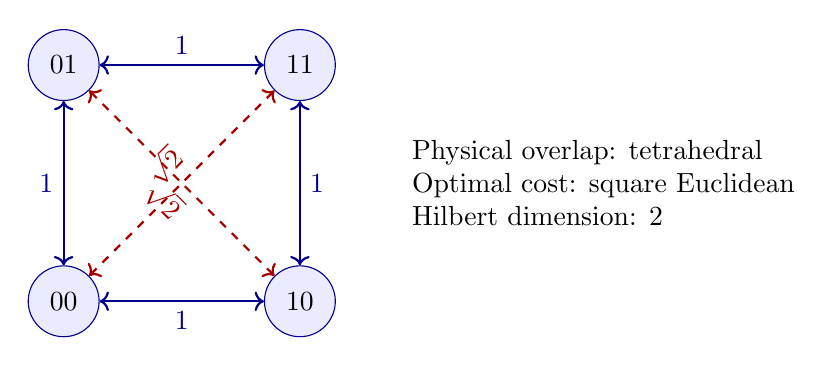
\begin{tikzpicture}[
  point/.style={circle,draw=blue!55!black,fill=blue!8,minimum size=9mm},
  edge/.style={-{Latex[length=2mm]},thick,blue!55!black},
  diag/.style={-{Latex[length=2mm]},thick,red!65!black,dashed}
]
\node[point] (a) at (0,0) {$00$};
\node[point] (b) at (3,0) {$10$};
\node[point] (c) at (0,3) {$01$};
\node[point] (d) at (3,3) {$11$};
\draw[edge,<->] (a)--node[below] {$1$}(b);
\draw[edge,<->] (a)--node[left] {$1$}(c);
\draw[edge,<->] (b)--node[right] {$1$}(d);
\draw[edge,<->] (c)--node[above] {$1$}(d);
\draw[diag,<->] (a)--node[sloped,above] {$\sqrt2$}(d);
\draw[diag,<->] (b)--node[sloped,below] {$\sqrt2$}(c);
\node[align=left,anchor=west] at (4.3,1.5) {
Physical overlap: tetrahedral\\
Optimal cost: square Euclidean\\
Hilbert dimension: $2$
};
\end{tikzpicture}
\caption{The smallest nondegenerate example. State geometry is tetrahedral,
but the action-cost geometry is exactly the Euclidean unit square.}
\label{fig:pauli-square}
\end{figure}

The Schoenberg matrix of \cref{eq:pauli-cost} is positive semidefinite of rank
two and reconstructs $(0,0),(1,0),(0,1),(1,1)$. This is the cleanest
demonstration that hodological geometry need not reproduce ambient quantum
state geometry.

\subsection{Minimality and limitation}

Four points are the smallest repertoire containing a complete square cell.
A one-dimensional quantum system can imitate the square only by storing all
four states in an external automaton. A qubit is the smallest nontrivial
system with the projective Pauli $\Z_2^2$ orbit. The construction is exact,
but it closes after two steps in either direction and therefore does not scale
to an open $3\times3$ lattice.

\section{An exact open qubit lattice from irrational phases}
\label{sec:irrational}

\subsection{Definition of the orbit}

Take
\begin{equation}
 \ket{+}=\frac{\ket0+\ket1}{\sqrt2},\qquad
 U=\begin{pmatrix}1&0\\0&e^{i\alpha}\end{pmatrix},\qquad
 V=\begin{pmatrix}1&0\\0&e^{i\beta}\end{pmatrix}
 \label{eq:qubit-controls}
\end{equation}
with
\begin{equation}
 \alpha=\frac{2\pi}{9}+\epsilon\sqrt2,\qquad
 \beta=\frac{2\pi}{3}+\epsilon\sqrt3,\qquad
 \epsilon=10^{-2}.
 \label{eq:chosen-phases}
\end{equation}
The four cardinal actions are the single-Kraus instruments
$U,U^\dagger,V,V^\dagger$. Define nine goals
\begin{equation}
 G_{ij}:\quad
 \ket{\psi_{ij}}=U^iV^j\ket+,\qquad i,j\in\{0,1,2\}.
 \label{eq:nine-qubit-goals}
\end{equation}
These are nine distinct, nonorthogonal phases on the qubit equator.

\subsection{Orbit--stabilizer viewpoint}

Let an action group or semigroup $\Gamma$ act on a fiducial ray. Its
projective stabilizer is
\begin{equation}
 K_\psi=\{k\in\Gamma:\pi(k)\ket{\psi_0}\sim\ket{\psi_0}\}.
 \label{eq:stabilizer}
\end{equation}
The orbit is naturally labelled by the quotient $\Gamma/K_\psi$. If action
words have norm $\|\cdot\|_{\mathcal A}$, the induced cost of displacement
$\Delta$ is
\begin{equation}
 d_{\rm hod}(0,\Delta)
 =\min_{k\in K_\psi}\|\Delta+k\|_{\mathcal A}.
 \label{eq:quotient-metric}
\end{equation}
Faithfulness, $K_\psi=\{0\}$, preserves the whole word metric. On a finite
patch, trivial stabilizer is stronger than necessary: it is enough that no
stabilizer relation shortens any displacement in the patch difference set.

\begin{theorem}[Faithfulness of the irrational qubit orbit]
\label{thm:qubit-faithful}
The map
\begin{equation}
 (a,b)\longmapsto U^aV^b\ket+
\end{equation}
with \cref{eq:chosen-phases} is injective on rays for $(a,b)\in\Z^2$.
\end{theorem}

\begin{proof}
Suppose $U^aV^b\ket+\sim\ket+$. The coefficient of $\ket0$ is unchanged, so
the global phase must be one. Equality of the relative phase requires
\begin{equation}
 a\alpha+b\beta=2\pi m,\qquad a,b,m\in\Z.
 \label{eq:phase-equation}
\end{equation}
Substituting \cref{eq:chosen-phases},
\begin{equation}
 2\pi\left(\frac a9+\frac b3-m\right)
 +\epsilon(a\sqrt2+b\sqrt3)=0.
 \label{eq:transcendence-equation}
\end{equation}
The second term is algebraic. If the rational coefficient of $\pi$ were
nonzero, the equation would express $\pi$ as an algebraic number, contradicting
its transcendence. Therefore
\begin{equation}
 \frac a9+\frac b3-m=0,\qquad a\sqrt2+b\sqrt3=0.
\end{equation}
Squaring the second relation gives $2a^2=3b^2$. Unique prime factorization
forces $a=b=0$; then $m=0$. The stabilizer is trivial.
\end{proof}

\subsection{Exact Manhattan word metric}

Because $U$ and $V$ commute, every cardinal action word reduces to
$U^aV^b$. To move $G_{ij}$ to $G_{kl}$, faithfulness forces
\begin{equation}
 (a,b)=(k-i,l-j).
\end{equation}
Any word realizing this displacement contains at least $|a|$ horizontal and
$|b|$ vertical generators. The canonical word attains the bound, so
\begin{equation}
 \boxed{
 d_1(G_{ij},G_{kl})=|k-i|+|l-j|
 }.
 \label{eq:exact-manhattan}
\end{equation}
This is exactly the open $3\times3$ square-lattice graph metric, even though
all nine rays lie on a single Bloch circle.

\subsection{Sequence-language formulation}

For a fixed horizon $H$, goal $G_{ab}$ can be stated as the finite language
of action sequences whose signed $U$ and $V$ exponent totals equal $(a,b)$.
A DFA may track
\begin{equation}
 (n_U,n_V,t)\in[-H,H]^2\times\{0,\ldots,H\},
\end{equation}
with a dead state for illegal or overlong histories. Taking $H=4$ retains
every shortest transition among the nine goals.

Without a horizon, exact equality of two unbounded integer counters is not a
regular language. Calling it regular would silently introduce an infinite
memory. The physical orbit remains mathematically well defined, but a finite
agent needs either bounded tasks, approximate counters, or a different
recognition mechanism.

\subsection{Exact Euclidean distance with unit-cost instruments}

Cardinal actions give $L^1$ distance. For each nonzero patch displacement
$\delta=(a,b)$, define
\begin{equation}
 r_\delta=\sqrt{a^2+b^2},\qquad
 K_{\rm s}(\delta)=\sqrt{\frac1{r_\delta}}\,U^aV^b,\qquad
 K_{\rm f}(\delta)=\sqrt{1-\frac1{r_\delta}}\,I.
 \label{eq:qubit-euclidean-instrument}
\end{equation}
Every attempt costs one. Since nonzero integer displacements have
$r_\delta\ge1$, this is a valid instrument. Failure changes nothing; success
performs the exact displacement.

\begin{corollary}[Exact qubit Euclidean patch]
For the nine goals in \cref{eq:nine-qubit-goals}, optimal expected cost under
\cref{eq:qubit-euclidean-instrument} is
\begin{equation}
 \boxed{
 d_2(G_{ij},G_{kl})
 =\sqrt{(k-i)^2+(l-j)^2}
 }.
 \label{eq:qubit-euclidean}
\end{equation}
\end{corollary}

\begin{proof}
The direct displacement has geometric waiting time of mean $r_\delta$.
Any composite strategy with successful displacements
$\delta_1,\ldots,\delta_n$ has expected cost at least
\begin{equation}
 \sum_q\|\delta_q\|_2
 \ge\left\|\sum_q\delta_q\right\|_2
\end{equation}
by the Euclidean triangle inequality. The direct retry action is optimal.
This is also the specialization of \cref{thm:retry} to $\Z^2$.
\end{proof}

\begin{figure}[t]
\centering
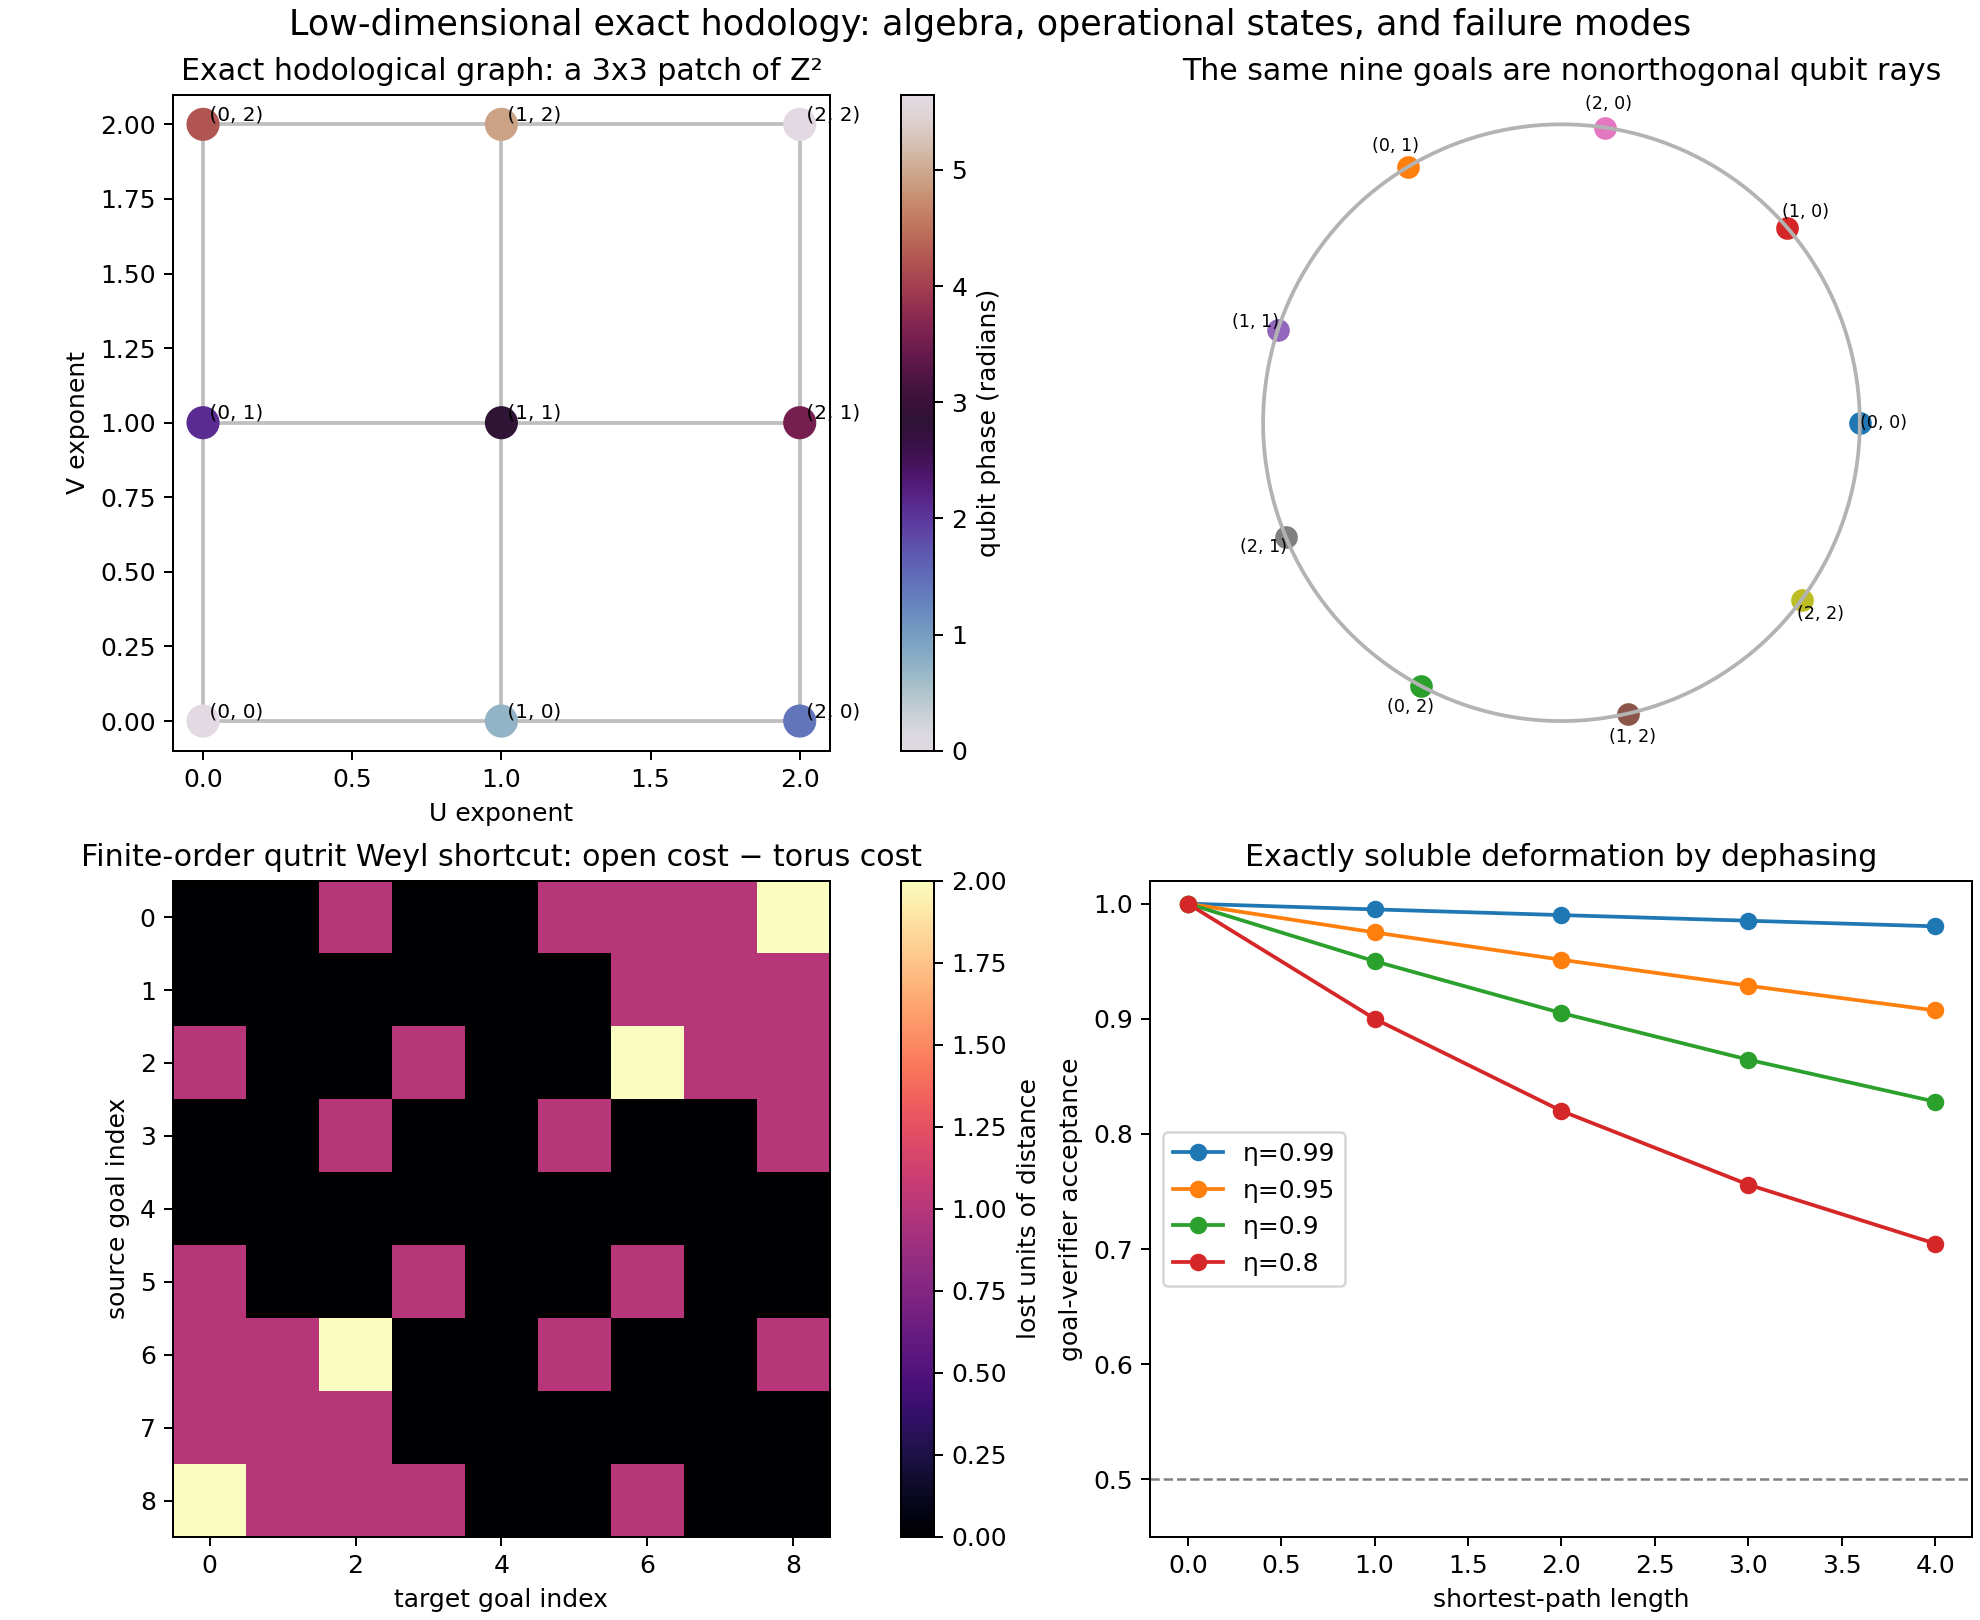
\includegraphics[width=\textwidth]{exact_qubit_lattice.png}
\caption{\textbf{Exact qubit construction and its failure modes.} The upper
panels show the open action-cost lattice and the nine physical rays on one
equatorial circle. The lower panels show finite-order qutrit wraparound and
the exactly soluble dephasing response.}
\label{fig:exact-qubit}
\end{figure}

\section{Recognition and robustness of the qubit construction}
\label{sec:qubit-robustness}

\subsection{One-sided verification is not exclusive localization}

Goal $G_{ij}$ has the yes/no projective test
\begin{equation}
 M_{\rm yes}=P_{ij}=\proj{\psi_{ij}},\qquad
 M_{\rm no}=I-P_{ij}.
\end{equation}
It accepts the exact target with probability one. A different goal is falsely
accepted with probability
\begin{equation}
 \Prob({\rm yes}\mid G_{kl})
 =|\braket{\psi_{ij}}{\psi_{kl}}|^2
 =\cos^2\left(
 \frac{(i-k)\alpha+(j-l)\beta}{2}
 \right).
 \label{eq:false-accept}
\end{equation}
For the chosen phases, minimum angular separation is $0.6352$ radians and
worst false acceptance is $0.9025$. Independent repreparations reduce a
one-sided error $q$ to $q^n$, but no finite number perfectly discriminates
nonorthogonal states.

Thus the exact theorem concerns history-labelled equality and control cost.
An experimental realization must include the resource needed to track history
or statistically recognize the target.

\subsection{Dense orbit and approximate stabilizers}

The irrational subgroup is dense on the equatorial phase circle. Hence
arbitrarily distant integer labels can produce arbitrarily close physical
rays. The inverse map from ray to $(a,b)$ is discontinuous. A useful
finite-resolution diagnostic is
\begin{equation}
 \ell_\varepsilon=
 \min\left\{|a|+|b|:\ (a,b)\ne(0,0),\
 1-|\bra+U^aV^b\ket+|^2\le\varepsilon\right\}.
 \label{eq:approx-stabilizer}
\end{equation}
Small $\ell_\varepsilon$ means that an approximate stabilizer creates a cheap
shortcut.

Enumerating exponent pairs through radius 18 gives:
\begin{table}[t]
\centering
\caption{Finite-tolerance shortcuts for the exact qubit construction.}
\label{tab:tolerance}
\begin{tabular}{rrrr}
\toprule
Allowed infidelity & shortened pairs & exact mean cost & tolerant mean cost\\
\midrule
$10^{-12}$ & $0.0000$ & $2.0000$ & $2.0000$\\
$10^{-5}$  & $0.0000$ & $2.0000$ & $2.0000$\\
$10^{-3}$  & $0.3056$ & $2.0000$ & $1.6111$\\
$10^{-2}$  & $0.3611$ & $2.0000$ & $1.5000$\\
\bottomrule
\end{tabular}
\end{table}
Exact injectivity therefore does not imply robust localization. Compactness
eventually defeats a large, noise-tolerant encoding without redundancy.

\subsection{Exactly soluble homogeneous dephasing}

After each intended unitary, apply
\begin{equation}
 \mathcal D_\eta(\rho)
 =\frac{1+\eta}{2}\rho+\frac{1-\eta}{2}Z\rho Z.
 \label{eq:dephasing}
\end{equation}
This channel multiplies qubit off-diagonal coherence by $\eta$. A path of
length $L$ multiplies it by $\eta^L$. The target projector therefore accepts
with probability
\begin{equation}
 \boxed{
 p_{\rm accept}(L,\eta)=\frac{1+\eta^L}{2}
 }.
 \label{eq:dephasing-solution}
\end{equation}
The noise is homogeneous and depends only on path length, so reliability
decays radially while the word geometry remains isotropic. Direction-dependent
dephasing after $U$ and $V$ would instead produce anisotropic, Finsler-like
difficulty.

\begin{proof}
The equatorial state has density matrix
\begin{equation}
 \rho_\varphi=\frac12
 \begin{pmatrix}1&e^{-i\varphi}\\e^{i\varphi}&1\end{pmatrix}.
\end{equation}
One application of \cref{eq:dephasing} multiplies the off-diagonal entries by
$\eta$; induction gives $\eta^L$. Overlap with the ideal target ray of the
same phase is the trace of their product, $(1+\eta^L)/2$.
\end{proof}

\section{A robust two-dimensional qutrit phase chart}
\label{sec:qutrit}

\subsection{Why a qutrit changes the problem}

A normalized qutrit pure state has two independent relative phases. Diagonal
unitaries modulo global phase form a two-torus, so two commuting control
directions can span a genuine two-dimensional state manifold. We now choose
the fiducial amplitudes and generators so that its local metric is exactly
isotropic.

Let
\begin{equation}
 \ket{\psi_0}
 =\sqrt{\frac38}\ket0+\frac12\ket1+\sqrt{\frac38}\ket2
 \label{eq:qutrit-fiducial}
\end{equation}
and define
\begin{equation}
 A=\diag(0,1,0),\qquad
 B=\diag\left(0,\frac12,1\right).
 \label{eq:qutrit-generators}
\end{equation}
They commute. The continuous orbit is
\begin{equation}
 \ket{\psi(\theta,\phi)}
 =e^{i(\theta A+\phi B)}\ket{\psi_0}.
 \label{eq:qutrit-continuous-orbit}
\end{equation}

\subsection{Deriving the Fubini--Study metric}

For a normalized pure-state family, the infinitesimal Fubini--Study line
element is
\begin{equation}
 ds^2=\braket{d\psi}{d\psi}
 -|\braket{\psi}{d\psi}|^2.
 \label{eq:fs-line}
\end{equation}
Differentiating \cref{eq:qutrit-continuous-orbit},
\begin{equation}
 \ket{d\psi}=i(A\,d\theta+B\,d\phi)\ket\psi.
\end{equation}
Substitution into \cref{eq:fs-line} gives the covariance form
\begin{equation}
 ds^2=
 \operatorname{Var}(A)d\theta^2+
 2\operatorname{Cov}(A,B)d\theta\,d\phi+
 \operatorname{Var}(B)d\phi^2.
 \label{eq:fs-covariance}
\end{equation}
Because $A$ and $B$ commute with the orbit unitaries, these moments are
constant everywhere on the orbit.

The fiducial probabilities in the computational basis are
$(3/8,1/4,3/8)$. Therefore
\begin{align}
 \langle A\rangle&=\frac14,&
 \langle A^2\rangle&=\frac14,&
 \operatorname{Var}(A)&=\frac14-\frac1{16}=\frac3{16},\nonumber\\
 \langle B\rangle&=\frac18+\frac38=\frac12,&
 \langle B^2\rangle&=\frac1{16}+\frac38=\frac7{16},&
 \operatorname{Var}(B)&=\frac7{16}-\frac14=\frac3{16},\nonumber\\
 \langle AB\rangle&=\frac18,&
 \operatorname{Cov}(A,B)&=\frac18-\frac14\frac12=0.
 \label{eq:qutrit-moments}
\end{align}
Hence
\begin{equation}
 \boxed{
 ds^2=\frac3{16}(d\theta^2+d\phi^2)
 }.
 \label{eq:isotropic-fs}
\end{equation}
The manifold is locally flat and square in these phase coordinates, up to one
common scale. A generic fiducial and pair of diagonal generators would produce
unequal variances or a cross term; the cancellation here is deliberate and
exact.

\subsection{A finite faithful orbit}

Choose an odd integer $m\ge5$ and set
\begin{equation}
 \epsilon_m=\frac{4\pi}{m},\qquad
 U=e^{i\epsilon_mA},\qquad
 V=e^{i\epsilon_mB}.
 \label{eq:qutrit-finite-controls}
\end{equation}
For the experiments, $m=11$. Both $U$ and $V$ have order $m$ and commute.

\begin{proposition}[Faithfulness for odd order]
\label{prop:qutrit-faithful}
For odd $m$, the projective orbit
\begin{equation}
 (x,y)\longmapsto U^xV^y\ket{\psi_0},
 \qquad (x,y)\in\Z_m^2,
 \label{eq:qutrit-finite-orbit}
\end{equation}
has $m^2$ distinct rays.
\end{proposition}

\begin{proof}
All three fiducial amplitudes are nonzero. If $U^xV^y$ stabilizes the ray, the
$\ket0$ component fixes the global phase to one. The phases on $\ket1$ and
$\ket2$ require
\begin{equation}
 2x+y\equiv0\pmod m,\qquad 2y\equiv0\pmod m.
\end{equation}
Because $m$ is odd, two is invertible modulo $m$. Thus $y=0$, then $x=0$.
\end{proof}

For $m=11$ the qutrit has 121 distinct, nonorthogonal orbit states. Their
number can exceed $d$ because they are not required to be one-shot
distinguishable.

\subsection{The square-torus control metric}

For a residue $r\in\Z_m$, let $\bar r$ be its centered representative in
\begin{equation}
 \left\{-\frac{m-1}{2},\ldots,\frac{m-1}{2}\right\}.
\end{equation}
Define
\begin{equation}
 d_m((x,y),(x',y'))
 =\sqrt{\bar r^2+\bar s^2},
 \quad r=x'-x,\quad s=y'-y.
 \label{eq:qutrit-torus-metric}
\end{equation}
This is a left-invariant control metric on the finite group $\Z_m^2$. Its
unit step is the common scale factored out of \cref{eq:isotropic-fs}.

For each nonzero centered displacement $(r,s)$, let
\begin{equation}
 W_{rs}=U^rV^s,\qquad
 L_{rs}=\sqrt{r^2+s^2},\qquad
 p_{rs}=\frac1{L_{rs}},
 \label{eq:qutrit-displacement}
\end{equation}
and use the instrument
\begin{equation}
 K_{\rm s}^{(r,s)}=\sqrt{p_{rs}}\,W_{rs},\qquad
 K_{\rm f}^{(r,s)}=\sqrt{1-p_{rs}}\,I_3.
 \label{eq:qutrit-retry}
\end{equation}
\Cref{thm:retry} proves that optimal expected cost is exactly
$d_m$.

\subsection{The exact open 3-by-3 chart}

Select
\begin{equation}
 \mathcal G_{3\times3}
 =\{(x,y):x,y\in\{0,1,2\}\}
 \label{eq:qutrit-patch}
\end{equation}
inside the $m=11$ orbit. Pairwise coordinate differences have magnitude at
most two, well below the wrap radius $5$. Therefore centered residues equal
ordinary differences, and
\begin{equation}
 \boxed{
 D((x,y),(x',y'))
 =\sqrt{(x-x')^2+(y-y')^2}
 }.
 \label{eq:qutrit-patch-distance}
\end{equation}
This is the exact Euclidean distance matrix of a square lattice. Its
Schoenberg Gram matrix has two positive eigenvalues, both six, and all other
eigenvalues vanish to numerical precision.

\begin{figure}[t]
\centering
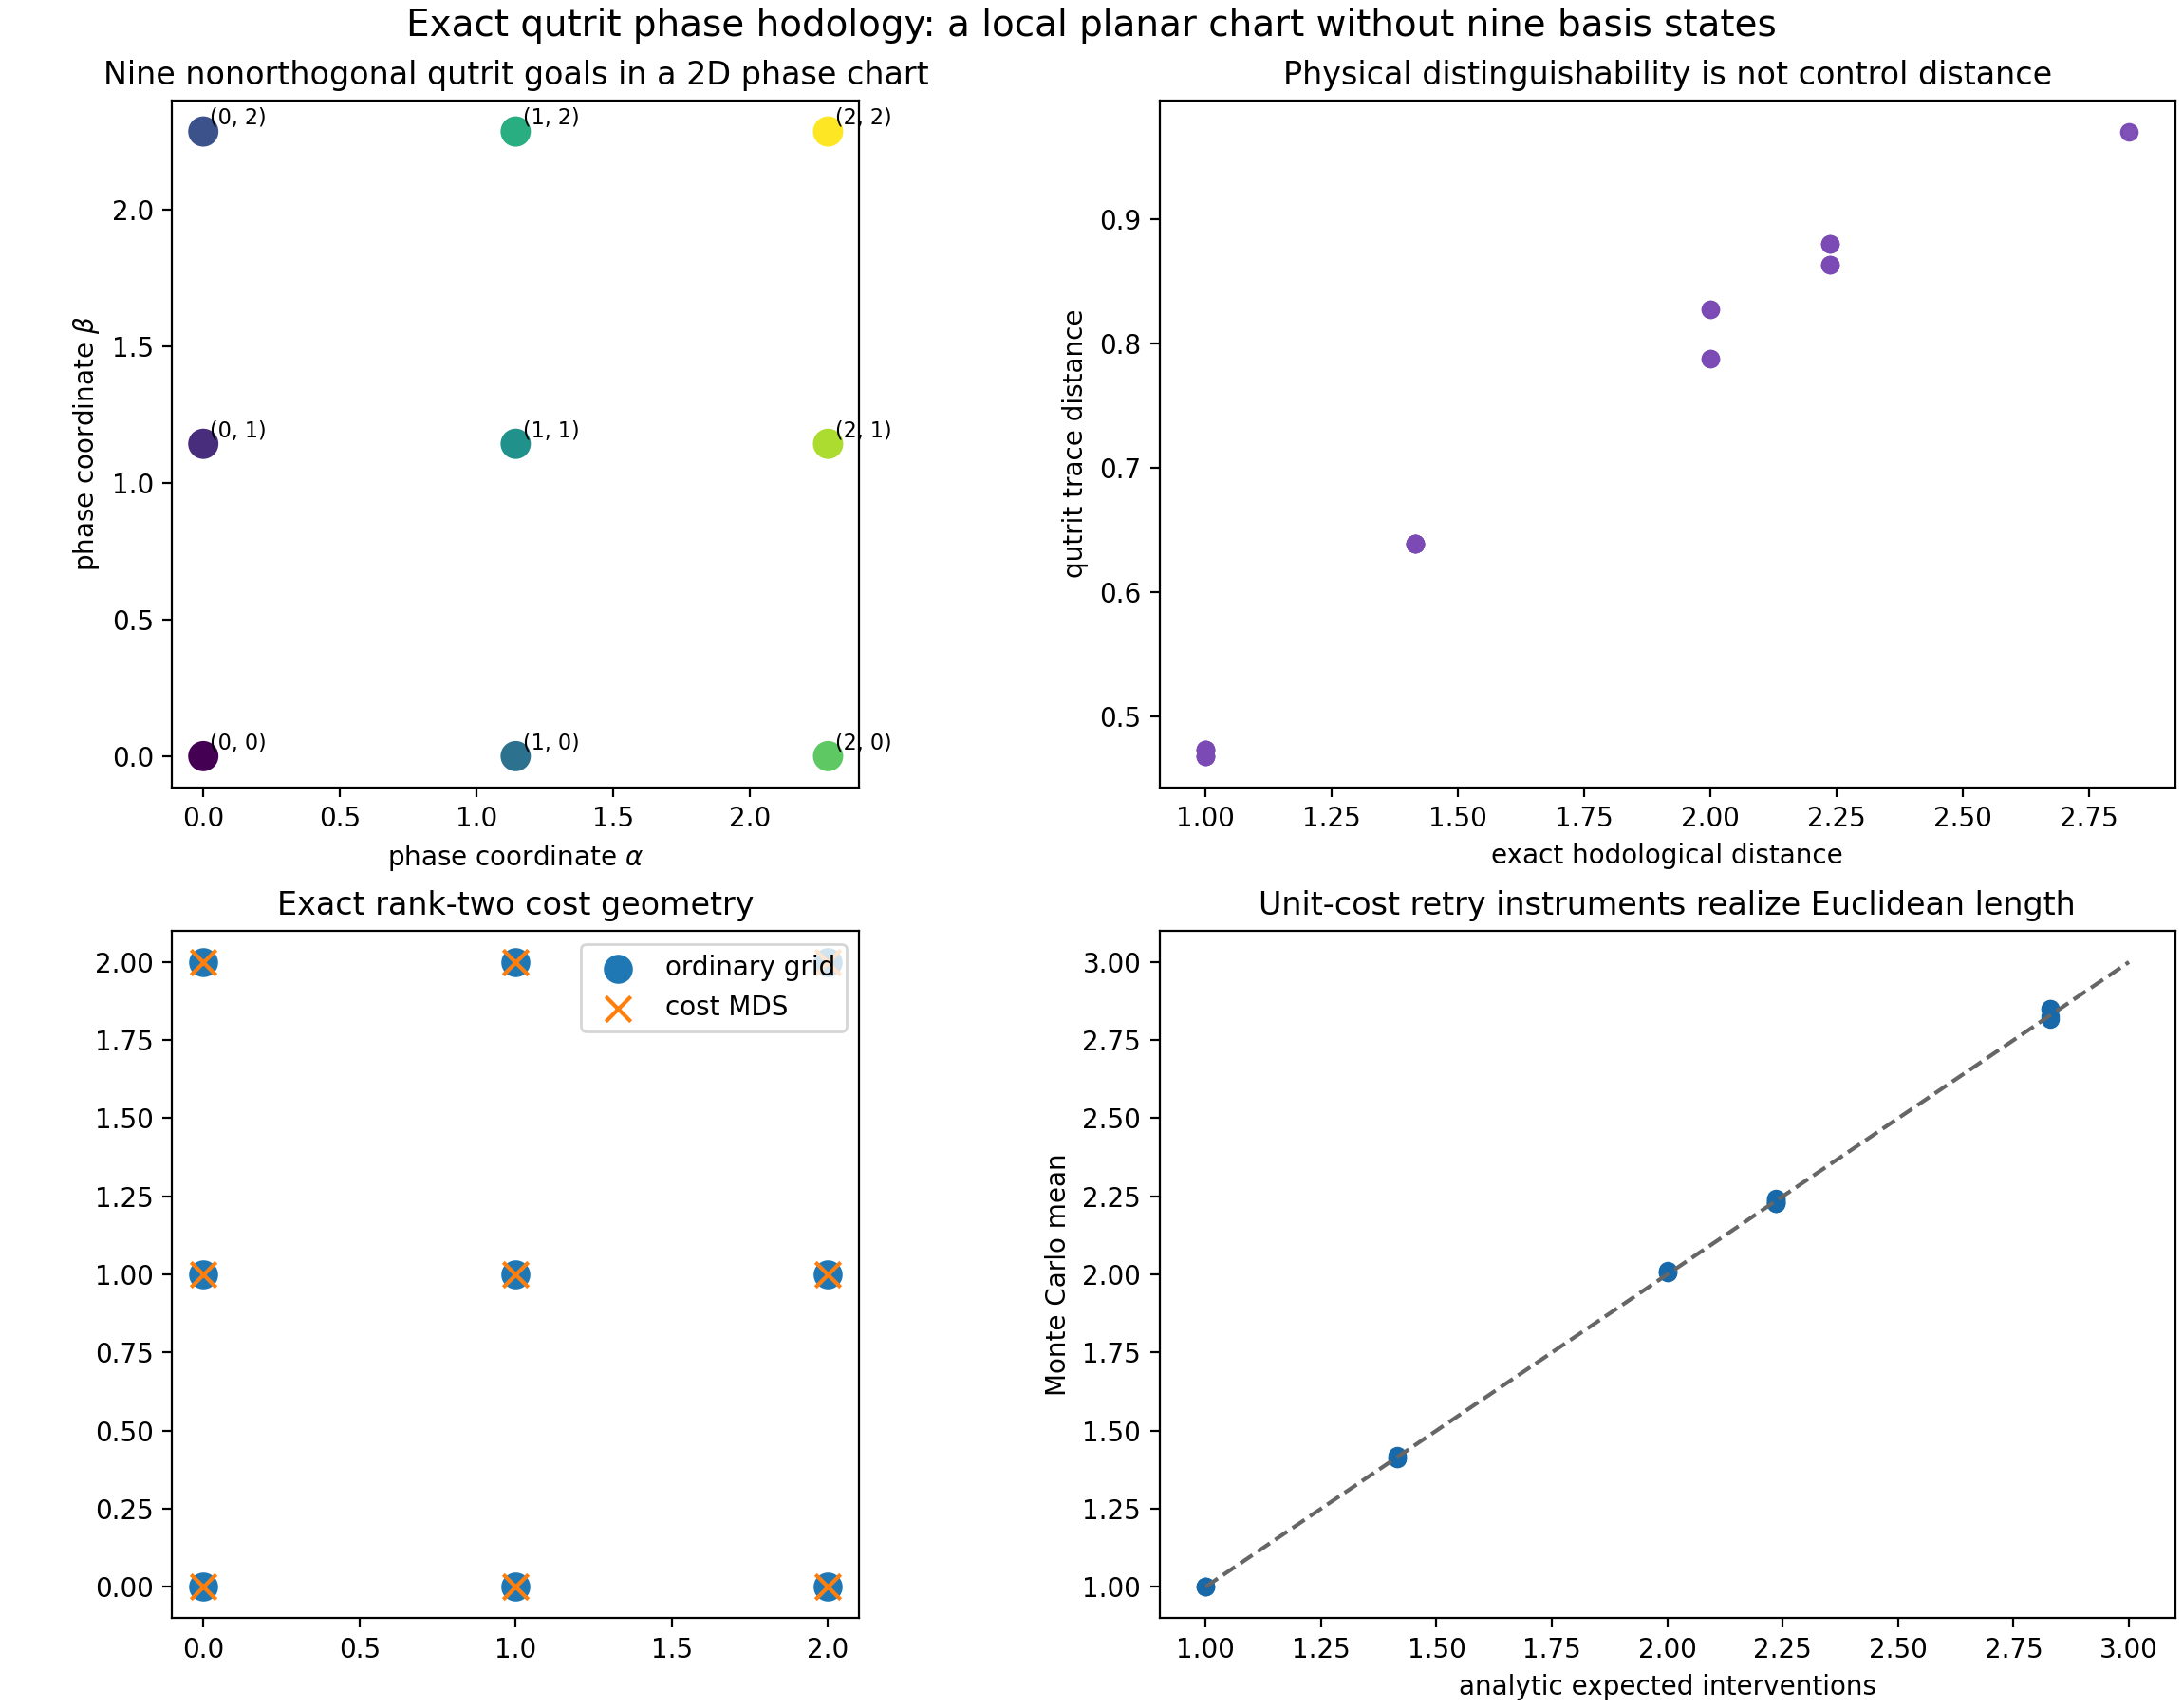
\includegraphics[width=\textwidth]{qutrit_phase_lattice.png}
\caption{\textbf{Exact qutrit phase construction.} The generator covariance
is isotropic; the finite order-11 orbit contains 121 separated rays; the
selected patch passes the exact Euclidean-distance and Bellman tests; and
Procrustes-aligned MDS coordinates coincide with the analytic grid.}
\label{fig:qutrit-phase}
\end{figure}

There is no physical wall around the patch. It is a local chart of a larger
periodic orbit. That is advantageous here: open-grid distances are obtained
without an orthogonal nine-state position register or a boundary-dependent
transition rule.

\subsection{Goal semantics and dead reckoning}

The clean exact monitor tracks successful displacement
\begin{equation}
 q_t=(x_t,y_t)\in\Z_m^2.
\end{equation}
With known initialization and no hidden disturbance,
\begin{equation}
 q_t=(x,y)\quad\Longrightarrow\quad \rho_t=\rho_{xy}.
 \label{eq:synchronization}
\end{equation}
Thus physical state and history monitor evolve in lockstep. This proves
existence, but it also allows dead reckoning: the agent can navigate from its
own observed success outcomes without inferring location from a separate
quantum probe.

The next operational test should hide the initial coordinate, insert
unobserved slips, and provide only weak nonorthogonal measurements. Then the
agent must infer a posterior over phase coordinates. Because the target states
are nonorthogonal, localization becomes a genuine Bayesian quantum filtering
problem while \cref{eq:qutrit-patch-distance} remains exact ground truth.

\section{Why the obvious qutrit Weyl construction is a torus}
\label{sec:weyl}

Define the generalized Pauli operators
\begin{equation}
 X\ket j=\ket{j+1\bmod3},\qquad
 Z\ket j=\omega^j\ket j,\qquad \omega=e^{2\pi i/3}.
 \label{eq:weyl}
\end{equation}
They satisfy $ZX=\omega XZ$, so their conjugation channels commute and their
projective classes generate $\Z_3^2$. A generic fiducial has nine orbit states.
This decisively refutes the claim that nine controlled states require
$d=9$.

It does not produce an open grid. Since $X^3=Z^3=I$, the stabilizer kernel is
$3\Z\times3\Z$. For example, open-grid displacement $(2,0)$ has length two,
but on the torus it equals $(-1,0)$ and takes one inverse action. In the
experiment, 16 of the 36 unordered goal pairs have strict shortcuts.

This is an algebraic fact, not a learning failure. Finite-order relations
quotient the intended translation lattice. The torus has two independent
translation directions and is intrinsically two-dimensional topologically,
but its nine-point shortest-path matrix is not an exact rank-two Euclidean
distance matrix. Open plane, periodic topology, and Euclidean metric are
different claims.

\section{Simulation results and exact audits}
\label{sec:experiments}

\subsection{Why simulate an exactly solved model?}

An exact construction still benefits from computation. Numerical checks can:
\begin{enumerate}
  \item catch implementation errors in Kraus operators and phase conventions;
  \item verify all source--goal pairs rather than only representative cases;
  \item test Monte Carlo convergence against analytic expectations;
  \item quantify finite-resolution behavior not visible in an exact proof;
  \item generate artifacts against which later learning agents can be tested.
\end{enumerate}
The simulation does not discover the theorem. It tries to falsify the code
that claims to instantiate it.

\subsection{Exact qubit audit}

All 81 ordered transitions among the nine qubit goals reach the analytic
target. The maximum floating-point terminal infidelity is
$6.7\times10^{-16}$. The Euclidean coordinate-distance error is zero.
For each of the 24 nonzero patch displacements, 50,000 geometric waiting times
were sampled, for 1.2 million samples in total. Maximum error of a sample mean
from the exact norm was 0.02897 interventions.

The same audit exposes the limitation: worst one-shot false acceptance is
0.9025, and at infidelity tolerance $10^{-3}$, 30.56\% of ordered nontrivial
pairs are shortened. The exact label geometry is much stronger than the
finite-resolution physical geometry.

\subsection{Exact qutrit audit}

\begin{table}[t]
\centering
\caption{Headline checks for the order-11 qutrit phase construction.}
\label{tab:qutrit-results}
\begin{tabular}{lr}
\toprule
Quantity & Result\\
\midrule
Hilbert dimension & $3$\\
Physical orbit states & $121$\\
Selected goal states & $9$\\
Fubini--Study covariance & $(3/16)I_2$\\
Minimum orbit Frobenius separation & $0.3450505$\\
Maximum Bellman residual & $8.88\times10^{-16}$\\
Maximum patch Euclidean error & $0$\\
Maximum MDS reconstruction error & $1.33\times10^{-15}$\\
Positive Schoenberg eigenvalues & $6,\ 6$\\
Control/trace-distance Pearson correlation & $0.988921$\\
Maximum waiting-time Monte Carlo error & $0.023733$\\
\bottomrule
\end{tabular}
\end{table}

The control/trace correlation is high because this is a small isotropic chart,
but the two metrics are conceptually different. Control cost is set by
instruments and expected attempts. Trace distance is set by statistical
distinguishability of physical states. Exact equality is neither assumed nor
observed.

\subsection{A dialectical reading of the evidence}

The results answer a sequence of progressively sharper objections:
\begin{description}[style=nextline]
 \item[Objection: nine goals require nine dimensions.]
 False. Both the qubit and qutrit constructions have nine distinct controlled
 goals.
 \item[Objection: perhaps the grid is only a fitted picture.]
 False for the cost matrices. Bellman and Schoenberg conditions prove the
 exact results.
 \item[Objection: perhaps any goal automaton could do this.]
 Correct in general. The identity-system control in
 \cref{prop:automaton} shows why physical orbit and memory provenance must be
 reported.
 \item[Objection: the qubit orbit is a physical plane.]
 False. It is dense on one phase circle. Its two-dimensionality is in the
 faithful action/history labels.
 \item[Objection: the qutrit Weyl orbit is the desired open plane.]
 False. It wraps into a torus.
 \item[Objection: the qutrit phase construction finally derives Euclidean
 distance.]
 Not yet. It derives an isotropic state manifold, but the inverse-distance
 retry probabilities still supply the Euclidean control norm.
\end{description}

\section{What exactly has emerged?}
\label{sec:interpretation}

\begin{table}[t]
\centering
\caption{The three exact constructions and the distinct claims they support.}
\label{tab:comparison}
\small
\begin{tabularx}{\textwidth}{lXXX}
\toprule
Construction & Exact achievement & Physical strength & Principal limitation\\
\midrule
Qubit Pauli square &
One Euclidean square cell &
Nontrivial projective qubit orbit &
Closes after two steps\\
Qubit irrational phase &
Open $\Z^2$ word metric and exact Euclidean patch cost &
Nine nonorthogonal controlled rays &
Dense one-dimensional orbit; fragile recognition\\
Qutrit order-11 phase &
Isotropic two-phase manifold and exact Euclidean local chart &
121 finite separated rays &
Euclidean retry law and macro-actions supplied\\
Qutrit Weyl orbit &
Exact homogeneous $\Z_3^2$ control topology &
Common finite projective group action &
Periodic torus, not an open Euclidean plane\\
\bottomrule
\end{tabularx}
\end{table}

The qubit answers the original cardinality question with the smallest possible
physical system. The qutrit answers the stronger manifold question. Neither
alone establishes that ordinary space generically emerges from quantum
control. Rather, they isolate what remains to be explained:
\begin{itemize}
 \item why a small local action family should select the Euclidean norm;
 \item how location is inferred without exact dead reckoning;
 \item why approximate stabilizers remain expensive under finite resolution;
 \item how local charts scale and agree on overlaps;
 \item how internal goal progress should be separated from spatial position.
\end{itemize}

\section{Toward necessary and sufficient conditions for space}
\label{sec:conditions}

There cannot be one useful classification theorem until the intended meaning
of space is fixed. Automaton universality makes an unrestricted statement
trivial. The following hierarchy separates exact finite geometry from the
stronger physical claim.

\subsection{Level I: exact Euclidean cost geometry}

For a finite operational MDP, the necessary-and-sufficient conditions are
already complete:
\begin{enumerate}
  \item every goal is properly reachable and the cost columns solve the
  Bellman equations;
  \item the all-pairs table satisfies symmetry and the metric axioms;
  \item its Schoenberg matrix is positive semidefinite of rank at most two or
  three.
\end{enumerate}
These conditions answer a precise mathematical question: whether optimal
difficulty is exactly the Euclidean distance of some point configuration.

\subsection{Level II: spatially consistent dynamics}

An arbitrary teleportation table can be tuned to have Euclidean costs. A
spatial interpretation additionally requires action-conditioned increments
to be local and reusable. If $x_i$ are recovered coordinates, then
\begin{equation}
 P_a(i,j)>0
 \quad\Longrightarrow\quad
 x_j-x_i\in S_a(i).
 \label{eq:increment-law}
\end{equation}
Away from boundaries, the distribution of increments under action $a$ should
be approximately independent of absolute position. This is translation
covariance. In a curved or inhomogeneous model, its controlled failure should
vary smoothly and be interpretable as a position-dependent metric or
connection.

\subsection{Level III: operationally identifiable place}

The coordinate must be inferable from the agent's available history to the
required accuracy. Exact one-shot identification obeys
\cref{prop:orthogonality}; sequential approximate identification does not.
Useful finite tests include localization error, posterior entropy at fixed
sensing budget, and discrimination performance after hidden disturbances.

\subsection{Level IV: low external-memory provenance}

The spatial coordinate should not live entirely in a hand-coded monitor.
Candidate diagnostics are:
\begin{itemize}
 \item minimal DFA size for exact goal recognition;
 \item predictive Hankel rank;
 \item recurrent-state dimension at fixed prediction error;
 \item performance after erasing action labels while retaining outcomes;
 \item performance after randomizing the unknown initial state;
 \item recovery after unobserved moves;
 \item comparison with an identity-channel or state-independent null
 instrument.
\end{itemize}
A useful hybrid control stores one coordinate in orthogonal qutrit basis
states and one in a three-state DFA. A correct provenance analysis should
identify one quantum-supported axis and one history-supported axis.

\subsection{Level V: robust manifold and bundle structure}

As goal repertoires grow, local dimension and metric tensors should converge.
Charts inferred from overlapping subsets should agree up to smooth coordinate
transformations. Approximate stabilizers should not create shortcuts within
the operational horizon. A useful invariant is the shortest nonzero word that
returns within fidelity tolerance $\varepsilon$ of its starting ray, as in
\cref{eq:approx-stabilizer}.

Only after a stable spatial base is established should internal degrees of
freedom be treated as fibers. If an internal state changes under transport
around a closed base loop, the learned transition law defines an operational
holonomy and possibly a discrete connection. The exact flat qutrit base is
valuable precisely because any measured holonomy can then be attributed to
the added coupling rather than uncertainty about base geometry.

\section{The most promising next construction}
\label{sec:future}

\subsection{Remove the displacement lookup table}

The exact retry catalog contains one action for every displacement class.
That makes the theorem transparent but places too much geometry in the action
repertoire. The strongest next experiment should retain the qutrit's isotropic
phase manifold while replacing the catalog by a small family of local
translation-covariant instruments.

An outer optimization can vary valid Kraus operators through Choi matrices or
Stinespring isometries. For each candidate environment, an inner exact planner
computes all-pairs Bellman costs. A possible objective is
\begin{equation}
\begin{split}
\mathcal L={}&
\lambda_B\,\mathcal L_{\rm Bellman}
+\lambda_-\,\|B_-\|_F^2
+\lambda_r\sum_{\ell>2}\lambda_\ell(B)^2\\
&+\lambda_{\rm iso}\,\mathcal L_{\rm anisotropy}
+\lambda_{\rm nl}\,\mathcal L_{\rm nonlocal}
+\lambda_{\rm tol}\,\mathcal L_{\rm tolerance}.
\end{split}
\label{eq:inverse-loss}
\end{equation}
Here $B_-$ is the negative part of the Schoenberg matrix, eigenvalues beyond
the first two penalize extra dimension, and the last terms discourage
nonlocal action semantics and fragile approximate stabilizers.

Training and evaluation displacements must be separated. A model that merely
memorizes the $3\times3$ table will fail at held-out radii and directions. A
genuinely emergent local metric should extrapolate.

\subsection{Derive length from continuous control energy}

There is also an analytic route that avoids retry macro-actions. Consider
\begin{equation}
 U(t)=e^{i(\theta(t)A+\phi(t)B)}.
\end{equation}
By \cref{eq:isotropic-fs}, Fubini--Study speed is
\begin{equation}
 v_{\rm FS}(t)=\frac{\sqrt3}{4}
 \sqrt{\dot\theta(t)^2+\dot\phi(t)^2}.
\end{equation}
If action cost is integrated speed,
\begin{equation}
 C[\theta,\phi]=
 \frac{\sqrt3}{4}\int_0^T
 \sqrt{\dot\theta^2+\dot\phi^2}\,dt,
 \label{eq:path-length}
\end{equation}
then minimizing cost gives straight phase paths and Euclidean geodesic
length. Discretizing this variational principle could make the metric arise
from local control energy rather than inverse-distance success probabilities.

\subsection{Make localization genuinely predictive}

After removing the lookup table, hide the initial phase coordinate and add
unobserved random slips. Provide only weak qutrit measurements whose
statistics vary smoothly across the orbit. A recurrent agent must then learn:
\begin{enumerate}
 \item a posterior or predictive state from measurement history;
 \item a local action model;
 \item goal-conditioned values;
 \item an atlas inferred from learned all-pairs costs.
\end{enumerate}
The exact phase chart supplies ground truth for separating model-estimation,
belief, planning, and execution error.

\section{Reproduction}
\label{sec:reproduction}

Run from the directory containing this document:
\begin{verbatim}
python -m unittest discover -s tests -v
python -m unittest discover -s search -p 'test_*.py' -v
MPLBACKEND=Agg python run_exact_experiments.py
MPLBACKEND=Agg python run_qutrit_phase_experiments.py
MPLBACKEND=Agg python search/search_low_dimensional.py
latexmk -pdf -interaction=nonstopmode \
  -halt-on-error EXACT_LOW_DIMENSIONAL_HODOLOGY.tex
\end{verbatim}

The exact-construction tests verify Kraus completeness, all 81 canonical qubit
transitions, Manhattan word distance, bounded sequence goals, Euclidean
macro-actions, geometric waiting time, qutrit wraparound, dephasing, qutrit
faithfulness, Fubini--Study isotropy, Bellman residuals, and Schoenberg rank.
The skeptical-search tests add automaton nulls, qutrit POVMs, toroidal Bellman
costs, qubit tangent patches, and quantum counter backaction.

Primary artifacts are:
\begin{description}[style=nextline]
 \item[\texttt{results/all\_pairs.csv}]
 Every ordered exact qubit source--goal transition.
 \item[\texttt{results/finite\_tolerance.csv}]
 Approximate-stabilizer shortcut audit.
 \item[\texttt{results/dephasing\_validation.csv}]
 Analytic and Monte Carlo values of \cref{eq:dephasing-solution}.
 \item[\texttt{results/euclidean\_waiting\_validation.csv}]
 Geometric waiting means for 1.2 million samples.
 \item[\texttt{results/qutrit-phase/summary.json}]
 Qutrit covariance, separation, Bellman, Schoenberg, and MDS checks.
\end{description}

\section{Conclusion}

Low Hilbert dimension does not count goals. A qubit can carry a faithful
action of $\Z^2$ and therefore an exact open lattice word metric; a qutrit can
carry a smooth, finite-resolution two-dimensional phase manifold. What low
dimension does constrain is perfect simultaneous recognition and robust
localization.

The exact constructions make several distinctions unavoidable. Physical state
geometry is not control geometry. A two-generator topology is not
automatically a Euclidean metric. A history coordinate is not automatically a
physical coordinate. A zero-stress distance matrix is not automatically a
local space. Bellman and Schoenberg conditions solve the finite cost-geometry
problem, while action covariance, recognition, memory provenance, and
robustness determine whether the result deserves a spatial interpretation.

The qutrit phase chart is the strongest present starting point. It supplies a
genuine isotropic two-dimensional quantum manifold, a finite separated orbit,
and an exactly solved goal geometry. The remaining challenge is no longer
whether such geometry is mathematically possible. It is to explain why a small
physically natural family of local quantum interventions should select a
noise-stable Euclidean metric that an agent can reconstruct from experience.

\appendix

\section{Worked Bellman check for a retry action}
\label{app:bellman}

Suppose the current point is $x$, the goal is $g$, and action $h$ succeeds
with probability $p=1/r$, where $r=d_G(e,h)$. Let
$V(x)=d_G(x,g)$. Its one-step value is
\begin{align}
 Q_h(x)
 &=1+\left(1-\frac1r\right)V(x)+\frac1rV(hx)\nonumber\\
 &=V(x)+1-\frac{V(x)-V(hx)}r.
 \label{eq:worked-bellman}
\end{align}
The triangle inequality gives $V(x)-V(hx)\le r$, hence
$Q_h(x)\ge V(x)$. If $h=gx^{-1}$, then $V(hx)=0$ and $r=V(x)$, so equality
holds. This one line contains both halves of optimality: every action is
bounded below by the metric, and the direct displacement attains it.

\section{Worked Schoenberg check for the unit square}
\label{app:square}

For points $(0,0),(1,0),(0,1),(1,1)$, use the distance matrix in
\cref{eq:pauli-cost}. Double centering its squared entries gives
\begin{equation}
B=
\begin{pmatrix}
\frac12&0&0&-\frac12\\
0&\frac12&-\frac12&0\\
0&-\frac12&\frac12&0\\
-\frac12&0&0&\frac12
\end{pmatrix}.
\label{eq:square-gram}
\end{equation}
Its eigenvalues are $1,1,0,0$: it is positive semidefinite of rank two.
The two positive eigenvectors recover a rotated and centered version of the
unit square. This is why rank, not visual inspection, certifies intrinsic
dimension.

\section{Notation and interpretive checklist}

\begin{tabularx}{\textwidth}{lX}
\toprule
Symbol & Meaning\\
\midrule
$d$ & Hilbert-space dimension\\
$\rho$ & Hidden or externally represented density operator\\
$h_t$ & Observable action--outcome history\\
$q_t$ & Explicit goal-progress or displacement monitor state\\
$D(i,g)$ & Optimal expected intervention cost\\
$D_{\rm tr}$ & Trace distance between physical states\\
$d_{\rm FS}$ & Fubini--Study distance or line element\\
$B$ & Double-centered Schoenberg Gram matrix\\
$K_\psi$ & Projective stabilizer of the fiducial ray\\
$U,V$ & Controlled phase translations\\
$K_{\rm s},K_{\rm f}$ & Success and failure Kraus operators\\
\bottomrule
\end{tabularx}

\medskip
Before interpreting any low-dimensional goal embedding, ask:
\begin{enumerate}
 \item What is the physical Hilbert dimension?
 \item What classical or recurrent memory recognizes the goal?
 \item Can different coordinates be distinguished by future quantum
 experiments?
 \item Does the proposed cost solve the Bellman equations?
 \item Does its Schoenberg matrix have the claimed rank and sign?
 \item Are action increments local and translation covariant?
 \item Does geometry survive unknown starts, hidden slips, and finite
 measurement tolerance?
 \item Is Euclidean length derived or inserted into action probabilities?
\end{enumerate}
\begin{thebibliography}{99}

\bibitem{bellman1957}
R.~Bellman, \emph{Dynamic Programming}
(Princeton University Press, 1957).

\bibitem{puterman1994}
M.~L. Puterman, \emph{Markov Decision Processes:
Discrete Stochastic Dynamic Programming}
(Wiley, 1994). \doi{10.1002/9780470316887}.

\bibitem{bertsekas1991}
D.~P. Bertsekas and J.~N. Tsitsiklis,
“An analysis of stochastic shortest path problems,”
\emph{Mathematics of Operations Research} 16, 580--595 (1991).
\doi{10.1287/moor.16.3.580}.

\bibitem{schoenberg1935}
I.~J. Schoenberg,
“Remarks to Maurice Fr\'echet's article
\emph{Sur la d\'efinition axiomatique d'une classe d'espaces distanci\'es
vectoriellement applicable sur l'espace de Hilbert},”
\emph{Annals of Mathematics} 36, 724--732 (1935).
\doi{10.2307/1968654}.

\bibitem{gower1966}
J.~C. Gower,
“Some distance properties of latent root and vector methods used in
multivariate analysis,”
\emph{Biometrika} 53, 325--338 (1966).
\doi{10.1093/biomet/53.3-4.325}.

\bibitem{nielsen2010}
M.~A. Nielsen and I.~L. Chuang,
\emph{Quantum Computation and Quantum Information},
10th anniversary ed. (Cambridge University Press, 2010).
\doi{10.1017/CBO9780511976667}.

\bibitem{bengtsson2017}
I.~Bengtsson and K.~\.{Z}yczkowski,
\emph{Geometry of Quantum States}, 2nd ed.
(Cambridge University Press, 2017).
\doi{10.1017/9781139207010}.

\bibitem{holevo2011}
A.~S. Holevo,
\emph{Probabilistic and Statistical Aspects of Quantum Theory},
2nd English ed. (Edizioni della Normale, 2011).
\doi{10.1007/978-88-7642-378-9}.

\bibitem{kraus1983}
K.~Kraus, \emph{States, Effects, and Operations}
(Springer, 1983). \doi{10.1007/3-540-12732-1}.

\end{thebibliography}

\end{document}
